\newcommand{\sscale}{.6}
\newcommand{\sscaler}{.3}
\begin{tikzpicture}[scale=\sscale]	
	%The picture of the hole with the desciption of phiin and phoout
	\newcommand{\arrowlength}{1 cm}
	\begin{scope}[xshift=-4 cm,yshift=0 cm]
		%The spectra
		\node at (0,0) {\includegraphics[scale=\sscale]{Figs_Friction/PolarForSi.pdf}};
		%The hole
		\newcommand{\hcent}{1 cm}
		\begin{scope}[xshift=-.9 cm,yshift=10.15 cm,>=stealth]
			\node at (0,0) {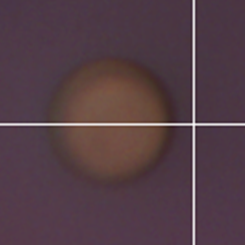
\includegraphics[scale=\sscaler ]{Figs_Friction/PolarPicture.png}};
			\draw[red,ultra thick,->] (\hcent-\arrowlength/2,-.03 cm) -- +(\arrowlength,0)  node[anchor=south west,fill=white]{$\phi_{in}$};
			\draw[green,ultra thick,->] (\hcent,-.03 cm) +(45:-\arrowlength/2) -- +(45:\arrowlength/2) node[anchor=south east, fill=white]{$\phi_{out}$};
		\end{scope}
	\end{scope}
	
	%The figure of the oscillating areas
	\begin{scope}[xshift=4 cm,yshift=0 cm]
		\node at (0,0) {\includegraphics[scale=\sscale]{Figs_Friction/ForSi_Areas.pdf}};
	\end{scope}
	
	\node at (.7,3) {\textbf{b}};
	\node at (-7,12.5) {\textbf{a}};
\end{tikzpicture}